\documentclass[10 pt,usenames,dvipsnames, oneside]{article}
\usepackage{../../../modelo-ensino-medio}



\begin{document}

\begin{center}
  \begin{minipage}[l]{3cm}

\includegraphics[width=2cm]{logo}    
\end{minipage}\hfill
\begin{minipage}[r]{.8\textwidth}
 {\Large \scshape Atividade: Variação do Dólar}  
\end{minipage}
\end{center}
\vspace{.2cm}

\ifdefined\prof
%Habilidades da BNCC
% \begin{objetivos}
% \item 
% \end{objetivos}

%Caixa do Para o Professor
\begin{goals}
%Objetivos específicos
\begin{enumerate}
\item Aplicar as inequações do segundo grau em contextos de economia.
\item Compreender geometricamente uma inequação de segundo grau.
\item Resolver algébrica e geometricamente uma inequação do segundo grau.
\end{enumerate}

\tcblower

%Orientações e sugestões
Professor, lembre ao aluno que a variação do Dólar em relação ao Real é descrito pela função dada no exercício apenas nesse dia, portanto, ao responder ao item $c)$ ele deve atentar que que o tempo não pode ser negativo nem maior que $24$, pois ambos os casos representariam outros dias.
\end{goals}

\bigskip
\begin{center}
{\large \scshape Atividade}
\end{center}
\fi

A cotação cambial do Dólar é um importante atributo para qualquer país e impacta vários indicadores econômicos, como inflação, balança comercial, dívida externa entre outros. 

\begin{figure}[H]
\centering
\noindent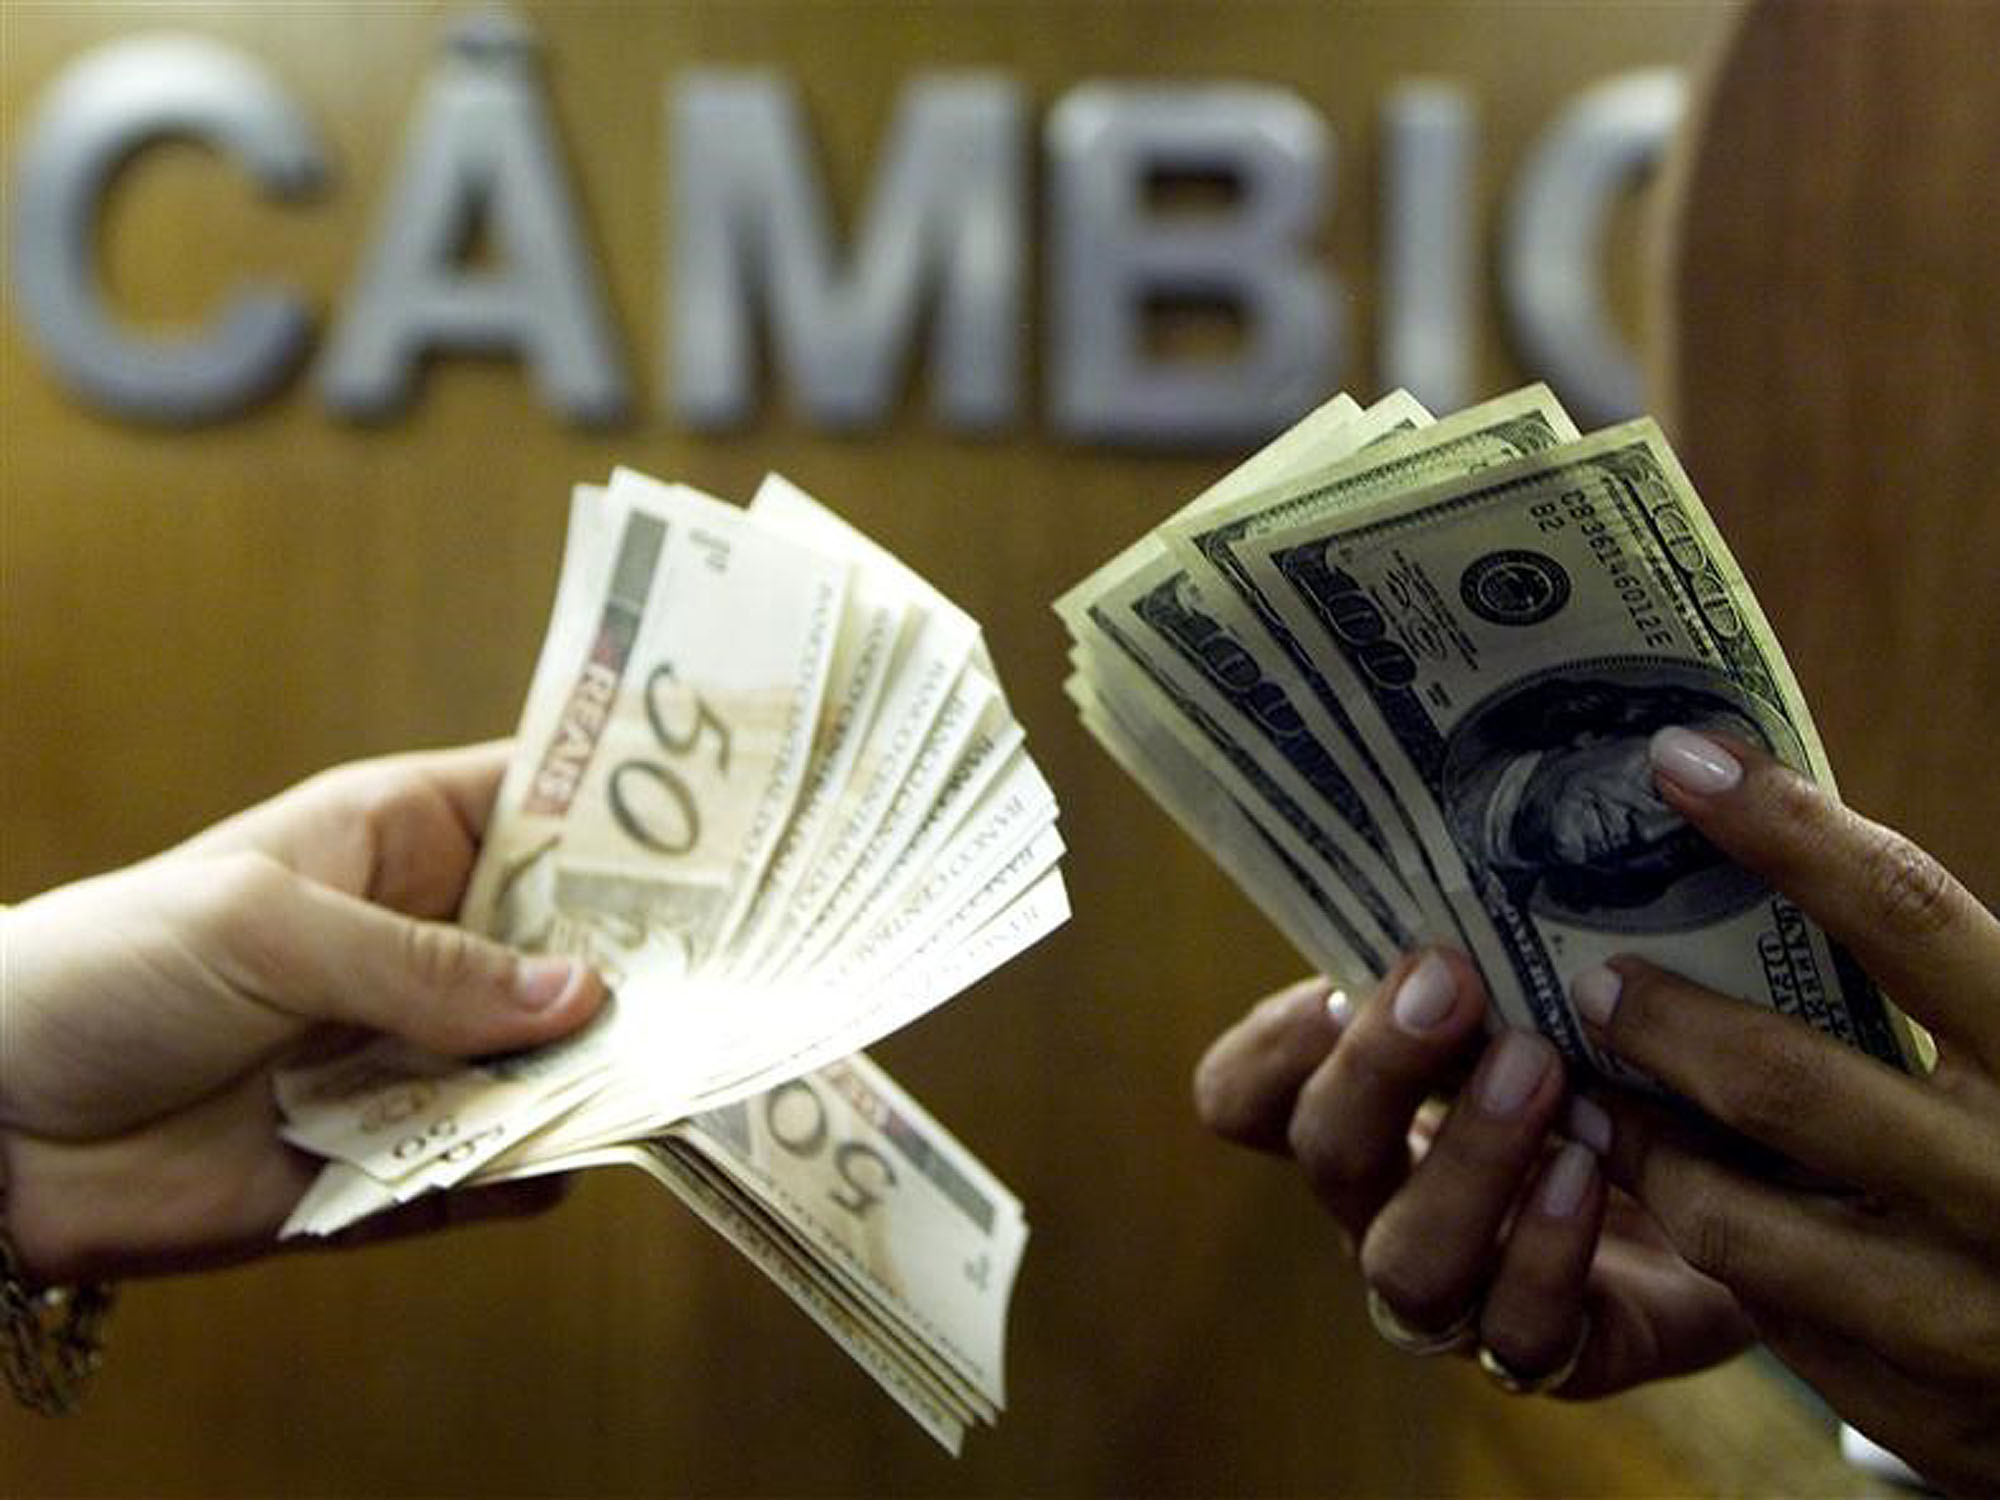
\includegraphics[width=200bp]{dolar}
\end{figure}

Suponha que em um determinado dia, a variação percentual $y$ do Dólar, frente o Real, tenha sido descrita pela seguinte função:
$$
y = -0,02t^2 + 0,3t, \ \ \ 9 \leq t \leq 17, 
$$
onde $t$ é medido em horas. Quando a variação percentual do Dólar é positiva, a moeda americana está se valorizando em relação ao Real, enquanto que quando esta variação é negativa, o dólar está se desvalorizando em relação ao Real.

\begin{enumerate}

\item{} Faça um esboço do gráfico da função $y = f(t)$ que descreve a variação percentual do dólar em função do tempo, no dia informado no enunciado;

\item{} Em qual período desse dia o dólar se valoriza em relação à nossa moeda? 

\item{} Em qual período desse dia o dólar se desvaloriza em relação ao Real?

\item{} Escreva algebricamente as perguntas dos itens \titem{b)} e \titem{c)};

\end{enumerate}

\ifdefined\prof
\begin{solucao}

\begin{enumerate}\setcounter{enumi}{1}
\item A partir das $0$hrs até às $15$hrs.
\item A partir das $15$hrs até o fim do dia.
\item O item $b)$ é representado por $f(t)=-0.002t^2-0.3t>0.$ O $c)$ fica $f(t)=-0.002t^2-0.3t<0. $
\end{enumerate}

\end{solucao}
\fi

\end{document}